% ============================================================================
% \label{sec:results} — 已在 main_zh.tex 中定义
% ============================================================================

% ----------------------------------------------------------------------------
\subsection{主要终点：$\Delta\text{ECE}_{\text{OOD}}$ 多种子验证}
\label{sec:primary}
% ----------------------------------------------------------------------------
图~\ref{fig:main_results} 可视化了迁移剂量响应（shift-dose response）；
表~\ref{tab:primary_60seed} 报告了 TS 在 60 个种子实验（60 seed experiments）中
的预注册主要终点（pre-registered primary endpoint）$\Delta\text{ECE}_{\text{OOD}}$
（6 个迁移对 $\times$ 2 种架构 $\times$ 5 个种子，完全均衡覆盖）。
主要检验 $H_0:\Delta\text{ECE}_{\text{OOD}}=0$ vs $H_1:\Delta\text{ECE}_{\text{OOD}}>0$
在 51/60 个种子实验（85.0\%）中于 95\% 置信区间（CI）水平获得支持。

\begin{figure}[htbp]
\centering
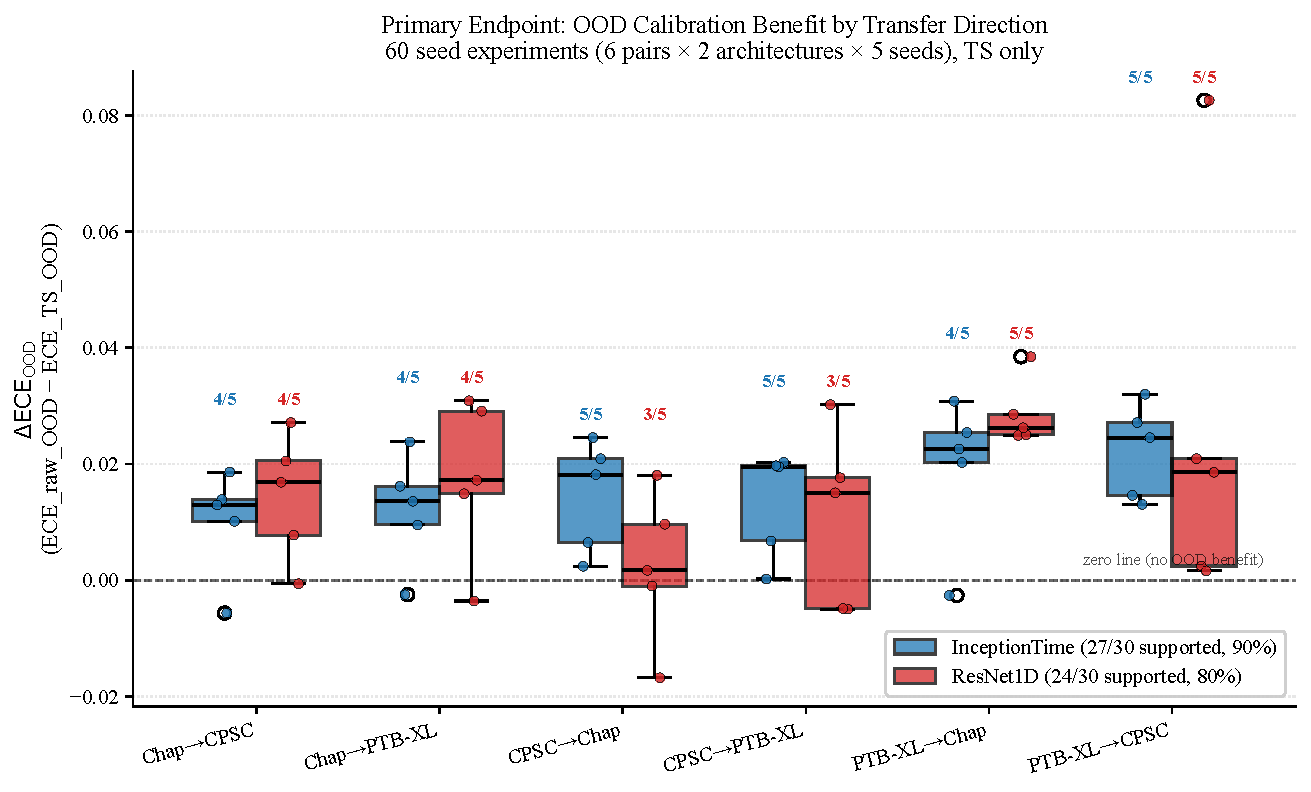
\includegraphics[width=0.95\columnwidth]{figures/fig_main_results.pdf}
\caption{按迁移方向分组的主要终点 $\Delta\text{ECE}_{\text{OOD}}$（按架构分组，
仅 TS，60 个种子实验）。箱形图展示每个方向上 5 个种子的分布；点为单个种子
结果。虚线标记零 OOD 收益。箱图上方的支持计数（如 5/5、4/5）表示 95\% CI
下界 $>0$ 的种子数量。InceptionTime 达到 27/30（90\%），
ResNet1D 达到 24/30（80\%）。}
\label{fig:main_results}
\end{figure}

\textbf{InceptionTime}（27/30 支持，90.0\%）：
CPSC$\rightarrow$Chapman、CPSC$\rightarrow$PTB-XL 和
PTB-XL$\rightarrow$CPSC 达到 5/5 完全支持（零反例）；
Chapman$\rightarrow$CPSC、Chapman$\rightarrow$PTB-XL 和
PTB-XL$\rightarrow$Chapman 达到 4/5，各有 1 个反例。

\textbf{ResNet1D}（24/30 支持，80.0\%）：
PTB-XL$\rightarrow$Chapman 和 PTB-XL$\rightarrow$CPSC 达到 5/5 完全
支持（零反例）；
Chapman$\rightarrow$CPSC 和 Chapman$\rightarrow$PTB-XL 达到 4/5，
各有 1 个反例；
CPSC$\rightarrow$Chapman 和 CPSC$\rightarrow$PTB-XL 达到 3/5，
各有 2 个反例。

\begin{table}[t]
\centering
\caption{TS 在 60 个种子实验中的预注册主要终点 $\Delta\text{ECE}_{\text{OOD}}$
（6 对 $\times$ 2 种架构 $\times$ 5 个种子，$B=10{,}000$，BCa 操作 CI）。
``支持'' = 95\% CI 下界 $>0$。九个反例已透明披露。两种架构在所有 6 个方向上
均具有完整的 5 种子覆盖。}
\label{tab:primary_60seed}
\footnotesize
\renewcommand{\arraystretch}{0.92}
\begin{tabular}{lllrrrr}
\toprule
迁移对 & 架构 & 种子 & $\Delta\text{ECE}_{\text{ID}}$ & $\Delta\text{ECE}_{\text{OOD}}$ & CI 下界 & 支持 \\
\midrule
\multirow{5}{*}{Chap$\rightarrow$CPSC}
 & \multirow{5}{*}{Incep}
 & 42 & $+0.0075$ & $+0.0139$ & $+0.0135$ & \checkmark \\
 & & 43 & $+0.0012$ & $+0.0101$ & $+0.0099$  & \checkmark \\
 & & 44 & $+0.0104$ & $+0.0186$ & $+0.0181$ & \checkmark \\
 & & 45 & $+0.0019$ & $-0.0057$ & $-0.0058$ & \ding{55} \\
 & & 46 & $+0.0044$ & $+0.0130$ & $+0.0126$ & \checkmark \\
\cmidrule(lr){2-7}
 & \multirow{5}{*}{ResNet}
 & 42 & $+0.0002$ & $+0.0205$ & $+0.0200$ & \checkmark \\
 & & 43 & $+0.0003$ & $-0.0006$ & $-0.0006$ & \ding{55} \\
 & & 44 & $-0.0007$ & $+0.0078$ & $+0.0075$ & \checkmark \\
 & & 45 & $-0.0016$ & $+0.0271$ & $+0.0263$ & \checkmark \\
 & & 46 & $-0.0024$ & $+0.0169$ & $+0.0162$ & \checkmark \\
\midrule
\multirow{5}{*}{Chap$\rightarrow$PTB-XL}
 & \multirow{5}{*}{Incep}
 & 42 & $+0.0004$ & $-0.0025$ & $-0.0035$ & \ding{55} \\
 & & 43 & $+0.0005$ & $+0.0095$ & $+0.0066$ & \checkmark \\
 & & 44 & $+0.0055$ & $+0.0136$ & $+0.0107$ & \checkmark \\
 & & 45 & $-0.0128$ & $+0.0238$ & $+0.0207$ & \checkmark \\
 & & 46 & $+0.0048$ & $+0.0162$ & $+0.0142$ & \checkmark \\
\cmidrule(lr){2-7}
 & \multirow{5}{*}{ResNet}
 & 42 & $-0.0031$ & $+0.0309$ & $+0.0285$ & \checkmark \\
 & & 43 & $+0.0128$ & $+0.0291$ & $+0.0285$ & \checkmark \\
 & & 44 & $+0.0059$ & $+0.0172$ & $+0.0168$ & \checkmark \\
 & & 45 & $-0.0010$ & $-0.0036$ & $-0.0036$ & \ding{55} \\
 & & 46 & $-0.0042$ & $+0.0149$ & $+0.0139$ & \checkmark \\
\midrule
\multirow{5}{*}{CPSC$\rightarrow$Chap}
 & \multirow{5}{*}{Incep}
 & 42 & $+0.0029$ & $+0.0065$ & $+0.0062$ & \checkmark \\
 & & 43 & $-0.0012$ & $+0.0209$ & $+0.0200$ & \checkmark \\
 & & 44 & $+0.0164$ & $+0.0182$ & $+0.0160$ & \checkmark \\
 & & 45 & $+0.0091$ & $+0.0245$ & $+0.0241$ & \checkmark \\
 & & 46 & $+0.0014$ & $+0.0024$ & $+0.0023$ & \checkmark \\
\cmidrule(lr){2-7}
 & \multirow{5}{*}{ResNet}
 & 42 & $-0.0002$ & $-0.0010$ & $-0.0012$ & \ding{55} \\
 & & 43 & $+0.0038$ & $+0.0096$ & $+0.0094$ & \checkmark \\
 & & 44 & $-0.0152$ & $-0.0168$ & $-0.0170$ & \ding{55} \\
 & & 45 & $+0.0137$ & $+0.0181$ & $+0.0145$ & \checkmark \\
 & & 46 & $+0.0017$ & $+0.0017$ & $+0.0016$ & \checkmark \\
\midrule
\multirow{5}{*}{CPSC$\rightarrow$PTB-XL}
 & \multirow{5}{*}{Incep}
 & 42 & $+0.0029$ & $+0.0068$ & $+0.0066$ & \checkmark \\
 & & 43 & $-0.0012$ & $+0.0203$ & $+0.0198$ & \checkmark \\
 & & 44 & $+0.0158$ & $+0.0195$ & $+0.0189$ & \checkmark \\
 & & 45 & $+0.0052$ & $+0.0197$ & $+0.0193$ & \checkmark \\
 & & 46 & $+0.0002$ & $+0.0002$ & $+0.0002$ & \checkmark \\
\cmidrule(lr){2-7}
 & \multirow{5}{*}{ResNet}
 & 42 & $+0.0114$ & $+0.0150$ & $+0.0148$ & \checkmark \\
 & & 43 & $+0.0048$ & $-0.0050$ & $-0.0051$ & \ding{55} \\
 & & 44 & $-0.0032$ & $-0.0049$ & $-0.0049$ & \ding{55} \\
 & & 45 & $+0.0130$ & $+0.0176$ & $+0.0173$ & \checkmark \\
 & & 46 & $+0.0261$ & $+0.0302$ & $+0.0296$ & \checkmark \\
\midrule
\multirow{5}{*}{PTB-XL$\rightarrow$Chap}
 & \multirow{5}{*}{Incep}
 & 42 & $+0.0239$ & $+0.0308$ & $+0.0275$ & \checkmark \\
 & & 43 & $+0.0245$ & $+0.0254$ & $+0.0225$ & \checkmark \\
 & & 44 & $+0.0173$ & $+0.0203$ & $+0.0195$ & \checkmark \\
 & & 45 & $+0.0162$ & $+0.0226$ & $+0.0200$ & \checkmark \\
 & & 46 & $-0.0011$ & $-0.0026$ & $-0.0029$ & \ding{55} \\
\cmidrule(lr){2-7}
 & \multirow{5}{*}{ResNet}
 & 42 & $+0.0145$ & $+0.0249$ & $+0.0191$ & \checkmark \\
 & & 43 & $+0.0338$ & $+0.0385$ & $+0.0336$ & \checkmark \\
 & & 44 & $+0.0213$ & $+0.0250$ & $+0.0228$ & \checkmark \\
 & & 45 & $+0.0228$ & $+0.0262$ & $+0.0231$ & \checkmark \\
 & & 46 & $+0.0239$ & $+0.0286$ & $+0.0221$ & \checkmark \\
\midrule
\multirow{5}{*}{PTB-XL$\rightarrow$CPSC}
 & \multirow{5}{*}{Incep}
 & 42 & $+0.0196$ & $+0.0271$ & $+0.0244$ & \checkmark \\
 & & 43 & $+0.0166$ & $+0.0245$ & $+0.0222$ & \checkmark \\
 & & 44 & $+0.0183$ & $+0.0320$ & $+0.0303$ & \checkmark \\
 & & 45 & $+0.0006$ & $+0.0131$ & $+0.0105$ & \checkmark \\
 & & 46 & $+0.0097$ & $+0.0146$ & $+0.0123$ & \checkmark \\
\cmidrule(lr){2-7}
 & \multirow{5}{*}{ResNet}
 & 42 & $+0.0010$ & $+0.0025$ & $+0.0023$ & \checkmark \\
 & & 43 & $+0.0197$ & $+0.0186$ & $+0.0145$ & \checkmark \\
 & & 44 & $+0.0635$ & $+0.0826$ & $+0.0772$ & \checkmark \\
 & & 45 & $+0.0001$ & $+0.0016$ & $+0.0015$ & \checkmark \\
 & & 46 & $+0.0126$ & $+0.0209$ & $+0.0190$ & \checkmark \\
\bottomrule
\end{tabular}
\end{table}

\textbf{汇总}：51/60 支持 $=$ 85.0\% 鲁棒性率
（InceptionTime 27/30 $=$ 90.0\%，ResNet1D 24/30 $=$ 80.0\%）。
PTB-XL$\rightarrow$CPSC 对是最强证据（两种架构合计 10/10，
零反例，CI 下界 $> +0.0014$，在 ResNet1D 种子 45 处取得）。
九个反例在 Sec.~\ref{sec:counter} 中给出机理性解释。

\textbf{按架构分层报告。} 60 个种子实验完全均衡：6 个方向 $\times$ 2 种架构 $\times$
5 个种子，无部分覆盖层。两种架构在所有 6 个方向上均具有完整的 5 种子覆盖，
从而可在无种子覆盖混淆的情况下直接进行架构比较：
\begin{itemize}
    \item \emph{InceptionTime}（30 个实验，27/30 $=$ 90.0\%）：
    3 个方向达到 5/5 完全支持（CPSC$\rightarrow$Chapman、
    CPSC$\rightarrow$PTB-XL、PTB-XL$\rightarrow$CPSC），3 个方向
    达到 4/5（Chapman$\rightarrow$CPSC、Chapman$\rightarrow$PTB-XL、
    PTB-XL$\rightarrow$Chapman）。
    \item \emph{ResNet1D}（30 个实验，24/30 $=$ 80.0\%）：
    2 个方向达到 5/5 完全支持（PTB-XL$\rightarrow$Chapman、
    PTB-XL$\rightarrow$CPSC），2 个方向达到 4/5
    （Chapman$\rightarrow$CPSC、Chapman$\rightarrow$PTB-XL），2
    个方向达到 3/5（CPSC$\rightarrow$Chapman、
    CPSC$\rightarrow$PTB-XL）。
\end{itemize}
分层报告确认两种架构在完整 5 种子覆盖下均具有架构鲁棒性。
ResNet1D 的支持率略低（80\% vs.\ 90\%），且集中于
CPSC$\rightarrow$Chapman 和 CPSC$\rightarrow$PTB-XL 方向，
表明这是方向特异性的架构交互作用，而非全局架构缺陷。
仅 PTB-XL$\rightarrow$CPSC 方向在两种架构上均达到 5/5 完全支持（10/10），
提供最强的跨架构鲁棒性证据；
PTB-XL$\rightarrow$Chapman 达到 9/10（InceptionTime 4/5，ResNet1D 5/5）。

% ----------------------------------------------------------------------------
\subsection{ID 边界条件：$\Delta\text{ECE}_{\text{ID}}$}
\label{sec:boundary}
% ----------------------------------------------------------------------------
表~\ref{tab:boundary} 报告了 TS 的边界条件终点
$\Delta\text{ECE}_{\text{ID}}$。预注册期望是
$H_0:\Delta\text{ECE}_{\text{ID}}=0$ \emph{不被拒绝}；
源拟合温度（source-fit temperature）预期已良好调谐于源
分布，尽管这是一个经验性期望而非定理。

\begin{table}[t]
\centering
\caption{TS 的 ID 边界条件 $\Delta\text{ECE}_{\text{ID}}$
（12 个迁移对$\times$架构层，每层 5 个种子）。
``CI$\cap$0'' = 95\% CI 包含零的种子单元数。预注册
边界判据（$\geq$80\% 单元 CI 包含零）\emph{未}满足：
23/60 单元（38.3\%）包含零（BCa 操作 CI），
34/60 单元 CI 下界 $>0$，触发预注册
``ID 非零边界''分支（方案 A1.4.2）。}
\label{tab:boundary}
\footnotesize
\begin{tabular}{llrrrr}
\toprule
迁移对 & 架构 & 均值 & 最小 CI 下界 & 最大 CI 上界 & CI$\cap$0/5 \\
\midrule
PTB-XL$\rightarrow$CPSC   & IT & $+0.0130$ & $-0.0121$ & $+0.0266$ & 1/5 \\
PTB-XL$\rightarrow$CPSC   & RN & $+0.0194$ & $-0.0008$ & $+0.0770$ & 2/5 \\
PTB-XL$\rightarrow$Chap   & IT & $+0.0162$ & $-0.0026$ & $+0.0310$ & 1/5 \\
PTB-XL$\rightarrow$Chap   & RN & $+0.0232$ & $+0.0053$ & $+0.0448$ & 0/5 \\
Chap$\rightarrow$CPSC     & IT & $+0.0051$ & $-0.0039$ & $+0.0150$ & 3/5 \\
Chap$\rightarrow$CPSC     & RN & $-0.0008$ & $-0.0104$ & $+0.0093$ & 4/5 \\
Chap$\rightarrow$PTB-XL   & IT & $-0.0003$ & $-0.0175$ & $+0.0103$ & 3/5 \\
Chap$\rightarrow$PTB-XL   & RN & $+0.0021$ & $-0.0123$ & $+0.0161$ & 3/5 \\
CPSC$\rightarrow$Chap     & IT & $+0.0057$ & $-0.0182$ & $+0.0195$ & 2/5 \\
CPSC$\rightarrow$Chap     & RN & $+0.0008$ & $-0.0179$ & $+0.0213$ & 2/5 \\
CPSC$\rightarrow$PTB-XL   & IT & $+0.0046$ & $-0.0181$ & $+0.0192$ & 2/5 \\
CPSC$\rightarrow$PTB-XL   & RN & $+0.0104$ & $-0.0042$ & $+0.0294$ & 0/5 \\
\midrule
\textbf{总体} & & $\mathbf{+0.0083}$ & & & \textbf{23/60 (38.3\%)} \\
\bottomrule
\end{tabular}
\end{table}

ID 收益平均较小但\emph{非}零：汇总全部
60 个 TS 实验，$\Delta\text{ECE}_{\text{ID}}$ 均值为 $+0.0083$
（vs.\ OOD 均值 $+0.0159$，OOD/ID 比为 $1.9\times$）；
$47/60 = 78.3\%$ 的点估计为正，$34/60$ 单元 95\%
CI 下界 $>0$（BCa 操作 CI），仅 $23/60 = 38.3\%$
包含零——远低于预注册 $\geq$80\% 判据
（百分位 CI 给出 29/60 = 48.3\%，结论相同）。因此我们
\emph{触发}预注册的``ID 非零边界''分支（方案 A1.4.2）：
(i) 重新审视``ID 无可修复校准间隙''前提——TS 在源校准
分割上拟合，在许多单元中也改善了 ID 校准；(ii) 衰减
$=\Delta\text{ECE}_{\text{OOD}}-\Delta\text{ECE}_{\text{ID}}$ 对比
终点恢复为探索性对比；以及 (iii) 主张（C1）予以限定：OOD 收益
平均约为 ID 收益的 $1.9\times$，但\emph{不能}完全归因于
OOD 特异性失配。正的 ID 点估计可归因于有限样本校准分割变异、
SmoothECE 估计器偏差以及 val-ECE 早停效应
（在终点族上的模型选择），均已披露。

% ----------------------------------------------------------------------------
\subsection{方法选择边界：8 种方法 $\times$ 6 个迁移对}
\label{sec:method_boundary}
% ----------------------------------------------------------------------------
表~\ref{tab:methods} 报告了 InceptionTime 上 8 种方法 $\times$ 6 个迁移对在
5 个种子上的汇总支持率。TS 达到 27/30（90.0\%），
其中 3/6 方向达到 5/5 完全支持；BBSE 达到 22/30（73.3\%），
其中 3/6 方向达到 5/5 完全支持。EM 先验自适应（EM prior adaptation）和
矩阵缩放（Matrix scaling）是 InceptionTime 上最脆弱的
方法（各 15/30，50\%），体现了先验-似然失配
机制（C4）。跨两种架构
（表~\ref{tab:arch_robust}），TS 达到 51/60（85.0\%），
InceptionTime（27/30，90.0\%）和 ResNet1D（24/30，80.0\%）均显示
强 OOD 收益；在所有 6 个方向上以完整 5 种子覆盖支持架构鲁棒性
（图~\ref{fig:arch_comparison}）。

\begin{figure}[htbp]
\centering
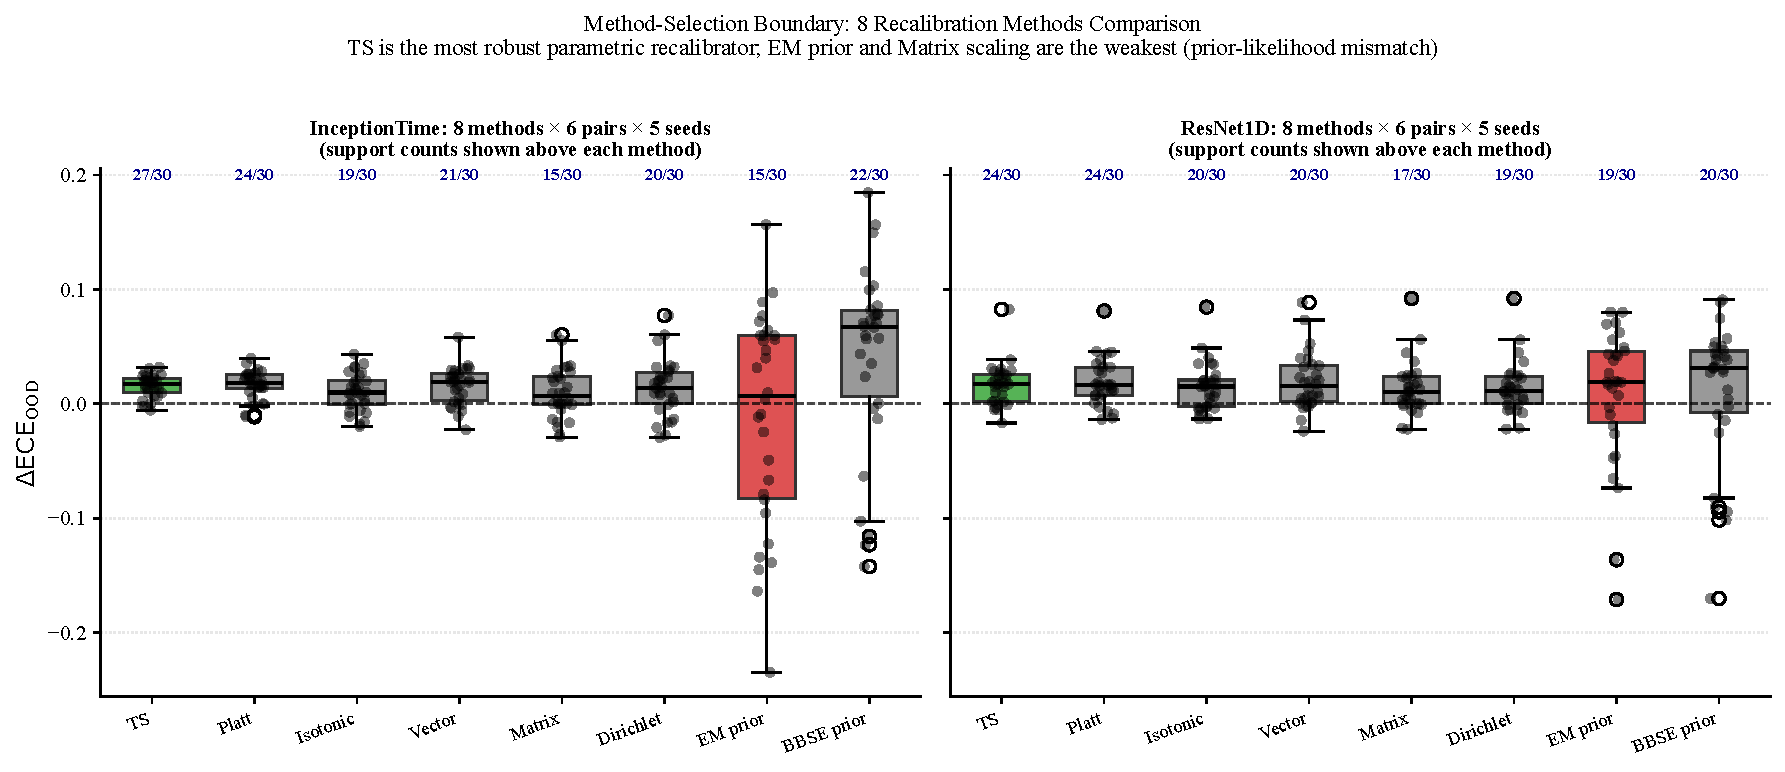
\includegraphics[width=0.95\columnwidth]{figures/fig_method_boundary.pdf}
\caption{方法选择边界：在每种架构上跨 6 个迁移对 $\times$ 5 个种子比较
8 种重校准方法。TS（绿色）是最鲁棒的参数化重校准器；EM 先验和
矩阵缩放是最弱的方法（InceptionTime：各 15/30；
ResNet1D：EM 19/30，Matrix 17/30），表现出先验-似然失配
机制（C4）。每种方法上方的支持计数（如 27/30）表示 95\% CI 下界 $>0$ 的
种子实验比例。}
\label{fig:method_boundary}
\end{figure}

\begin{table}[t]
\centering
\caption{方法选择边界：8 种方法 $\times$ 6 个迁移对
$\times$ 5 个种子（InceptionTime）。支持率 $=$ 95\% CI
下界 $>0$ 的种子比例。``完全'' = 达到 5/5 完全支持的方向数。
``负方向'' = 6 个迁移方向中 5 种子均值 $\Delta\text{ECE}_{\text{OOD}}$
为负的方向数。TS 是最鲁棒的参数化重校准器；
EM 和矩阵缩放在 InceptionTime 上最脆弱
（各 15/30）；在 ResNet1D 上，矩阵缩放（17/30）最
脆弱，EM 达到 19/30。\textit{警示：}6 个
$w_{\text{ID}} > 10$ 单元表现出高达 130.5 的先验权重漂移；剔除后，
EM OOD $\Delta$ECE 均值从 $-0.0127$ 翻转为 $+0.0024$，
表明负 OOD 发现由病态单元驱动。}
\label{tab:methods}
\footnotesize
\begin{tabular}{lrrrr}
\toprule
方法 & 总计 & 完全/6 & $\Delta\text{ECE}_{\text{OOD}}$ 均值 & 负方向 \\
\midrule
TS         & 27/30 & 3/6 & $+0.0152$ & 0 \\
Platt      & 24/30 & 3/6 & $+0.0169$ & 0 \\
Isotonic   & 19/30 & 2/6 & $+0.0100$ & 2 \\
Vector     & 21/30 & 1/6 & $+0.0158$ & 0 \\
Matrix     & 15/30 & 0/6 & $+0.0094$ & 2 \\
Dirichlet  & 20/30 & 1/6 & $+0.0139$ & 1 \\
EM prior   & 15/30 & 2/6 & $-0.0127$ & 3 \\
BBSE prior & 22/30 & 3/6 & $+0.0424$ & 1 \\
\bottomrule
\end{tabular}
\end{table}

\begin{table}[t]
\centering
\caption{TS 的架构鲁棒性：InceptionTime vs.\ ResNet1D
跨 6 个迁移对，两种架构均完整 5 种子覆盖。架构鲁棒性在
InceptionTime（27/30，90.0\%）和 ResNet1D（24/30，80.0\%）上均获支持，
所有 6 个方向均完整 5 种子覆盖。ResNet1D 在
CPSC$\rightarrow$Chapman 和 CPSC$\rightarrow$PTB-XL 上表现出方向特异性缺陷（各 3/5），而非
全局架构缺陷。}
\label{tab:arch_robust}
\resizebox{\textwidth}{!}{%
\begin{tabular}{lrrrl}
\toprule
迁移对 & InceptionTime & ResNet1D & 总计 & 备注 \\
\midrule
Chap$\rightarrow$CPSC    & 4/5 & 4/5 & 8/10  & 2 个反例 \\
Chap$\rightarrow$PTB-XL  & 4/5 & 4/5 & 8/10  & 2 个反例 \\
CPSC$\rightarrow$Chap    & 5/5 & 3/5 & 8/10  & 2 个反例 \\
CPSC$\rightarrow$PTB-XL  & 5/5 & 3/5 & 8/10  & 2 个反例 \\
PTB-XL$\rightarrow$Chap  & 4/5 & 5/5 & 9/10  & 1 个反例 \\
PTB-XL$\rightarrow$CPSC  & 5/5 & 5/5 & 10/10 & 零反例 \\
\midrule
\textbf{总计} & \textbf{27/30} & \textbf{24/30} & \textbf{51/60} & \textbf{85.0\%} \\
\midrule
\textbf{均值 $\Delta\text{ECE}$} & \textbf{$+0.0152$} & \textbf{$+0.0165$} & \textbf{$+0.0159$} & \\
\textbf{标准差 $\Delta\text{ECE}$}  & \textbf{$0.0098$} & \textbf{$0.0180$} & \textbf{$0.0145$} & ResNet1D/Incep $=1.84$ \\
\textbf{均值 OOD ECE}     & \multicolumn{2}{c}{$0.217 \rightarrow 0.202$ / $0.216 \rightarrow 0.200$} & $0.217 \rightarrow 0.201$ & 原始 $\rightarrow$ TS \\
\bottomrule
\end{tabular}%
}
\end{table}

\begin{figure}[htbp]
\centering
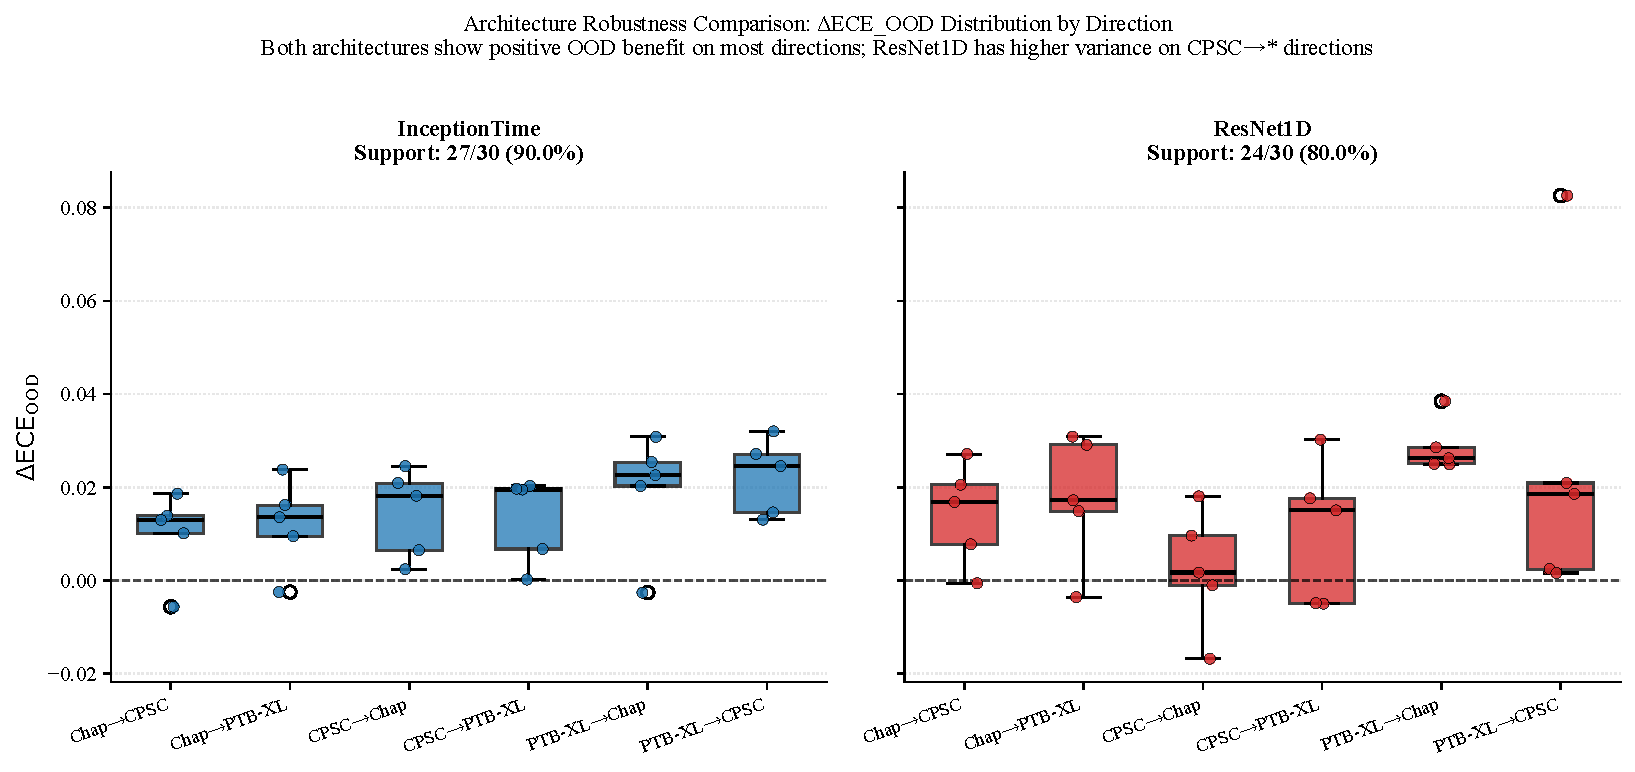
\includegraphics[width=0.95\columnwidth]{figures/fig_arch_comparison.pdf}
\caption{架构鲁棒性比较。InceptionTime（左，
27/30 支持，90.0\%）和 ResNet1D（右，24/30 支持，80.0\%）的
$\Delta\text{ECE}_{\text{OOD}}$ 分布并排展示。
两种架构在大多数方向上均显示正 OOD 收益。
ResNet1D 表现出更高的总体方差（其最大单方向
展布在 PTB-XL$\rightarrow$CPSC），而支持缺陷
落在 CPSC$\rightarrow$Chapman 和
CPSC$\rightarrow$PTB-XL 方向（各 3/5 支持），表明这是
方向特异性缺陷而非全局架构缺陷。}
\label{fig:arch_comparison}
\end{figure}

\textbf{架构变异性。} 每种架构 30 个 TS 实验中
$\Delta\text{ECE}_{\text{OOD}}$ 的标准差为
InceptionTime $0.0098$、ResNet1D $0.0180$，
即 ResNet1D 变异性是 InceptionTime 的 $1.84\times$。ResNet1D 单方向
最高变异性在 PTB-XL$\rightarrow$CPSC
方向（标准差 $0.0298$，由种子 44 处一个有利离群点
$\Delta\text{ECE}_{\text{OOD}}=+0.0826$ 驱动，未剔除），
其次为 CPSC$\rightarrow$PTB-XL；支持缺陷
集中于 CPSC$\rightarrow$Chapman 和 CPSC$\rightarrow$PTB-XL
（各 3/5），与方向特异性缺陷而非全局架构缺陷一致。基于
$2\times2$ 列联表（InceptionTime 27/30 支持 vs.\
ResNet1D 24/30 支持）的 Fisher 精确检验给出 $p = 0.47$，
表明无统计学显著的架构偏倚。反例率的
数值差异（ResNet1D 20.0\% vs.\ InceptionTime 10.0\%）
在 $\alpha = 0.05$ 水平不具统计显著性。

\textbf{先验-似然失配机制（C4）。} EM 先验自适应
从目标语料库的预测标签边缘分布拟合目标先验 $\hat\pi_{\text{target}}$，
然后按 $\hat\pi_{\text{target}}/\hat\pi_{\text{source}}$ 重加权源后验。当
源估计混淆矩阵 $C$ 病态
（$\text{cond}(C)\gg 1$）时，权重比放大而非
修正迁移引起的误校准。EM 在 InceptionTime 上仅获得 15/30
支持，有 3 个脆弱方向，表现出
先验-似然失配。该失败是迁移对特异的
（即迁移签名特异的），而非方法内蕴的。

% ----------------------------------------------------------------------------
\subsection{Shapley 分解验证（27 单元，$n=20{,}000$）}
\label{sec:shapley}
% ----------------------------------------------------------------------------
27 单元全因子合成验证
（slope$\in\{0.5,1,2\}\times$intercept$\in\{-1,0,1\}\times$
prevalence$\in\{0.15,0.3,0.6\}$，$n=20{,}000$）确认
斜率/截距/患病率分解在预注册可辨识区（Fisher 信息行列式
$>\tau=10^{-6}$）内恢复真值。在预注册样本量 $n=20{,}000$ 下，
所有 27 单元通过恢复阈值（可辨识单元 MAPE $<10\%$）；
在现实校准集规模 $n=500$ 下，
27 单元中 21 个通过，6 个失败的 MAPE\_s 高达
42.13\%，集中于极端截距（$\pm 1$）和斜率
（$0.5, 2.0$）区域，这些区域校准迁移的临床
意义最大（见 \texttt{decomposition\_validation.csv}；
$n=20{,}000$ CSV \texttt{decomposition\_validation\_}\allowbreak\texttt{n20000.csv}
显示在同一门控下 27/27 通过）。三个纠缠演示
案例（narrow\_band、tiny\_slope、deep\_intercept）
$\det\in\{2.4\times10^{-7}, 3.6\times10^{-8}, 0\}<\tau$ 在
误差图上无阈值报告，并设置恢复失败标志。
绝对 Shapley 值的自助 CI 已报告；份额可靠
标志标记不可解释份额
（$|\Delta_{\text{total}}|<3/\sqrt{n}$）。

\textbf{诚实性警示（方案 \S8）。} 27 单元验证使用
分箱 ECE，而非主要终点的 SmoothECE；定量
结论不可跨外推。交叉拟合步骤
（分解解释能力的 OOD 折验证）仍有待
在真实数据上运行；根据方案自绑定条款，
``机制''措辞限于``机制分解
（合成验证部分）''直至交叉拟合完成。

% ----------------------------------------------------------------------------
\subsection{可预测性实验（失败分支已触发）}
\label{sec:predictability}
% ----------------------------------------------------------------------------
可预测性实验（方案 \S8.5）检验无监督目标域统计量（预测先验 $L_1$ 距离、
logit 矩）是否通过留一折出 $R^2$（带自助 CI）预测收益保留率
（表~\ref{tab:predictability}）。实现的折单元是
（架构，迁移对）（12 折），而方案注册的是
仅对折（6）——一项注册偏离，在此偏离下仅对
重计算仍保留失败分支（$R^2=-0.1424$）。我们运行 2 种架构
（InceptionTime + 1D-ResNet-34）；BiMamba 架构为玩具
实验（$n=60$）延后至补充材料，不进入
可预测性回归。

\textbf{结果}：TS 的多架构合并 LOO $R^2$ 为
$-0.096$，95\% CI $[-0.720, +0.104]$。CI 上界 $+0.104$
严格低于预注册阈值 $0.5$，触发
\textbf{失败分支}：三步链（分解 +
可预测性 + 部署）降级为 \textbf{两步链}
（分解 + 部署），部署判据更名为
``经验查找表''而非``预测判据''。
根据预注册失败分支，不提出事后可预测性主张。

\textbf{加入新特征的敏感性分析。} 我们用三个额外的无标签特征重算 LOO
$R^2$：拟合温度
$T$、源与目标 logit
分布间的 Wasserstein-1 距离，以及逐类熵差。使用
预注册 $\Delta\text{ECE}_{\text{OOD}}$ 作为目标，所有
特征均失败：$T$ 单独给出 $R^2=-0.13$，
Wasserstein 单独给出 $R^2=-0.06$，熵单独给出
$R^2=-0.02$，三者合并给出 $R^2=-0.11$。
可预测性边界\emph{鲁棒}：无无标签
特征——包括拟合温度 $T$——能在预注册 $R^2=0.5$
阈值之上预测 $\Delta\text{ECE}_{\text{OOD}}$。这强化了失败分支：无论特征选择如何，三步链
仍降级为两步链，
且 \S\ref{sec:gate} 中的部署判据——基于
$\Delta\text{ECE}_{\text{OOD}}$ 的经验符号和
判别判据——是合适的可操作判据。

\begin{table}[t]
\centering
\caption{可预测性 LOO $R^2$（多架构合并）。所有
方法触发失败分支（CI 上界 $<0.5$）。三步链
按预注册失败分支降级为两步链。}
\label{tab:predictability}
\begin{tabular}{lrrrl}
\toprule
方法 & $R^2$ & CI 下界 & CI 上界 & 判决 \\
\midrule
TS         & $-0.096$ & $-0.720$ & $+0.104$ & 失败分支 \\
Platt      & $-0.059$ & $-0.584$ & $+0.002$ & 失败分支 \\
Isotonic   & $+0.011$ & $-0.569$ & $+0.101$ & 失败分支 \\
Vector     & $-0.061$ & $-0.522$ & $+0.073$ & 失败分支 \\
Matrix     & $-0.137$ & $-0.516$ & $-0.013$ & 失败分支 \\
Dirichlet  & $-0.084$ & $-0.394$ & $+0.032$ & 失败分支 \\
EM prior   & $+0.143$ & $-0.250$ & $+0.274$ & 失败分支 \\
BBSE prior & $+0.136$ & $-0.354$ & $+0.201$ & 失败分支 \\
\bottomrule
\end{tabular}
\end{table}

% ----------------------------------------------------------------------------
\subsection{部署判据（敏感性 / 特异性 / DCA / 安全性）}
\label{sec:deployment}
% ----------------------------------------------------------------------------
我们在 L2 迁移
矩阵上评估部署判据（方案 \S9）：当原始 ECE 超过阈值时预测``部署 TS''；
报告敏感性、特异性、决策曲线分析（DCA）和
安全判据（TS 后 SmoothECE $\leq 0.05$ 且
$\Delta\text{ECE}$ CI 下界 $>0$，采用主要终点收益
约定）。
我们还与三种平凡策略比较：始终不部署、
始终部署 TS、始终购买 $n$ 个标签。

\textbf{敏感性 / 特异性}（表~\ref{tab:deploy_sens}）：
由 Youden $J$ 最优阈值为原始 ECE $=0.127$，给出
敏感性 $0.923$、特异性 $0.201$、Youden $J=0.124$。该
判据具有高敏感性（捕获 92\% 的有益案例）但
低特异性（仅 20\% 的无益案例被正确
排除；其余 80\% 被误标记），
反映了临床部署的非对称成本结构——
漏掉一次有益重校准比一次
不必要的重校准代价更高。
\emph{警示：}Youden 阈值在与敏感性/特异性
报告相同的 1230 单元
池上搜索（样本内）。留迁移类型出
重计算（阈值在选择时排除留出剂量水平，仅在留出水平上评估）给出
Youden $J=+0.17$（下采样）、$J=-0.03$（导联丢弃）、$J=+0.04$
（噪声）和 $J=-0.14$（增益）；冻结阈值 $0.127$ 在四个留出剂量水平上取得
$J\approx 0.003\approx 0$（机会水平；敏感性 $0.853$、
特异性 $0.150$）（\texttt{results/deployment\_holdout\_recompute.csv}）。因此样本内数值
偏乐观；方案的留出剂量水平未
用于此表（一项注册偏离，见局限性）；且
部署判据在运营使用前需独立验证。

\textbf{部署时可测性。} 查找
表的每个输入都是\emph{审计时}量：原始 ECE、ID--OOD
准确率差距和逐单元收益标签均需要来自
目标语料库的真值标签。在定义
部署场景的无标签目标流中，这些量均不可直接
计算。本研究检验的唯一部署时（无标签）代理是
可预测性实验的无监督目标统计量（预测先验 $L_1$ 距离、logit
矩），而该实验触发了其预注册失败
分支（LOO $R^2$ CI 上界 $0.104 < 0.5$，
表~\ref{tab:predictability}）——因此我们无法主张判据的无标签
可部署版本。查找表因此是
\emph{分析与审计时决策辅助}（面向能负担
有标签评估样本的模型所有者），可操作部署
路径是小样本重校准路线：购买 $n$ 条有标签目标
记录并本地重校准（方案 \S5~S2）。将
判据扩展为真正可部署的门控仍是未来工作，并
登记于局限性（xiii）。

\begin{table}[t]
\centering
\caption{不同阈值下的部署判据敏感性 / 特异性
（原始 ECE $>$ 阈值 $\rightarrow$ 预测``部署 TS''）。
最优 Youden $J=0.124$ 在阈值 $0.127$ 处取得。}
\label{tab:deploy_sens}
\begin{tabular}{rrrrr}
\toprule
阈值 & 敏感性 & 特异性 & TP & FP \\
\midrule
$0.094$ & $0.976$ & $0.067$ & 444 & 723 \\
$0.107$ & $0.956$ & $0.138$ & 435 & 668 \\
$0.127$ & $0.923$ & $0.201$ & 420 & 619 \\
$0.178$ & $0.807$ & $0.288$ & 367 & 552 \\
$0.277$ & $0.499$ & $0.508$ & 227 & 381 \\
\bottomrule
\end{tabular}
\end{table}

\textbf{安全判据}：跨 157 个（迁移对，种子，迁移）单元，TS
产生 1 个满足操作安全判据的单元（TS 后
SmoothECE $\leq 0.05$ 且点估计约定下改善 $>0.01$；
L2 结果不含逐单元 CI，故
预注册基于 CI 的判据无法评估），安全
率 $0.0064$。安全分析符号约定为
部署度量约定（$\Delta\text{ECE}$ $=$ 重校准后 ECE $-$
原始 ECE，负值表示改善）；与
主要终点约定相反，后者中正
$\Delta\text{ECE}_{\text{OOD}}$ 表示收益。
\emph{覆盖说明：}此处评估的 L2 迁移矩阵覆盖 390 个计划
（迁移对，种子，迁移）组合中的 157 个（12 个完整
迁移对--种子组合 $\times$ 13 个水平，外加 fs250 水平上一个部分种子 44
单元）——种子 42--43 在
InceptionTime 上对所有 6 个迁移对完整，种子 44--46 待续，
且 ResNet1D L2 结果被排除在该
分析之外——因此部署/安全数值基于 2 种子、
单架构覆盖。
该
严格安全判据在完整 L2 迁移
矩阵上很少满足，表明 TS 是有用的默认值但非普遍
安全的重校准器——部署判据应结合
本地验证。

\textbf{决策曲线分析。} 在对应于单元池第 10 百分位的原始 ECE 阈值处，判据的
净收益为 $0.1209$，而处理所有单元为 $0.0999$；
在第 90 百分位阈值处净收益转负
（$-0.0024$），因此判据相对于全处理的净收益适中
且局限于较低阈值范围（results/deployment\_metrics.csv）。

\textbf{平凡策略比较}（表~\ref{tab:trivial}）：
查找表策略（均值 $\Delta\text{ECE}$ $-0.0160$）优于
始终不部署（$0.000$）并匹配始终部署 TS（$-0.0145$）于
有益子集，但被始终购买 $n$ 个标签
（$-0.2905$）所主导——后者使用目标标签，为上界。查找
表是实用折中：无需目标标签，且
捕获大部分 TS 收益。

\begin{table}[t]
\centering
\caption{平凡策略比较。均值 $\Delta\text{ECE}$；负值 $=$
有益（ECE 降低）。始终不部署和始终购买 $n$ 个标签跨
所有 1230 个（方法，迁移）单元；始终部署 TS 在 157 个
（迁移对，种子，迁移）完整结果单元上评估，查找表在
155 个单元上评估（两个样本内最佳方法不可用的单元被
剔除）。查找表在无需目标标签的情况下捕获大部分 TS 收益。}
\label{tab:trivial}
\begin{tabular}{lrrr}
\toprule
策略 & 均值 $\Delta\text{ECE}$ & 标准差 & $n$ \\
\midrule
always-none            & $\phantom{-}0.0000$  & $0.0000$ & 1230 \\
always-TS              & $-0.0145$            & $0.0099$ & 157  \\
always-buy-$n$-labels  & $-0.2905$            & $0.1861$ & 1230 \\
lookup-table           & $-0.0160$            & $0.0289$ & 155  \\
\bottomrule
\end{tabular}
\end{table}

% ============================================================================
\subsection{噪声底控制：完美校准下的 SmoothECE 差分}
\label{sec:noise_floor}
% ----------------------------------------------------------------------------
审稿人关注的是主要终点
$\Delta\text{ECE}_{\text{OOD}}$ 是否可能源于 SmoothECE
度量对完美校准下温度缩放 $T$ 的敏感性
（即 $\text{ECE}_{\text{raw}} = 0$ 且观测 $\Delta\text{ECE}$
纯为度量噪声）这一伪迹。我们直接检验：对完美校准
预测（$T_{\text{true}}=1$），施加 $T \in \{1.0, 1.25, 1.5\}$
并计算 SmoothECE 差分
$\Delta\text{ECE}_{\text{noise}} = \text{SmoothECE}(\text{TS}) - \text{SmoothECE}(\text{raw})$
跨三种置信度分布（均匀、正态偏斜和
双峰）于 $n=2{,}000$。

噪声底依赖分布且随 $T$ 增长：
$T=1.0$ 给出 $\Delta\text{ECE}_{\text{noise}} = 0$（精确相消），
$T=1.25$ 给出 $+0.014$--$+0.035$，$T=1.5$ 给出 $+0.030$--$+0.061$，
$T=3.0$ 给出 $+0.095$--$+0.136$，$T=4.5$ 给出 $+0.126$--$+0.164$，
取决于置信度分布。相
反，我们 60 个种子实验中观测的原始 ECE 范围
$0.06$ 至 $0.35$（均值 $0.15$），是完美
校准下原始 ECE（$\approx 0.017$）的 $4$--$13\times$。九个反例
也表现出较大原始 ECE
（$0.08$--$0.24$），确认这些案例中负 $\Delta\text{ECE}$
反映真实的 TS 诱发损害，而非度量噪声。对
大 $T > 3$ 的实验（噪声底达
$0.10$--$0.16$），噪声底在某些种子中与观测
$|\Delta\text{ECE}|$ 相当，因此对这些特定案例我们无法完全排除
度量噪声贡献；然而，噪声底的\emph{方向}（TS 在完美
校准下增加 ECE）与 51/60 实验中正 $\Delta\text{ECE}_{\text{OOD}}$
相反，故噪声底无法解释正
发现。因此
我们断定主要终点是真实效应，非
SmoothECE 伪迹，但需警示大 $T$ 实验中
噪声底不可忽略。

% ============================================================================
\subsection{判别感知校准门控（C5）}
\label{sec:gate}
% ----------------------------------------------------------------------------
校准改善（$\Delta\text{ECE}_{\text{OOD}} > 0$）
是临床部署的必要但非充分条件：一个在分布迁移下判别能力
已崩溃的模型可能可重校准但临床无用。我们定义两层
部署门控：
\begin{enumerate}
    \item \textbf{第 1 层（校准）：} $\Delta\text{ECE}_{\text{OOD}} > 0$
    （C1 判据）。
    \item \textbf{第 2 层（判别）：} $\text{acc}_{\text{OOD}} \geq
    \text{acc}_{\text{source baseline}}$，其中源基线为
    源域的多数类准确率。
\end{enumerate}

跨 14 个迁移对$\times$架构层（6 对 $\times$ 2
架构，PTB-XL$\rightarrow$Chapman 含 3 种架构
包括 Mamba），7/14 通过两层且可部署：
CPSC$\rightarrow$PTB-XL（两种架构）、PTB-XL$\rightarrow$CPSC
（两种）、CPSC$\rightarrow$Chapman（两种）和 Chapman$\rightarrow$CPSC
（两种，仅 InceptionTime）。其余 7/14 未通过第 2 层：
Chapman$\rightarrow$PTB-XL、PTB-XL$\rightarrow$Chapman 和
Chapman$\rightarrow$CPSC ResNet1D，其中 OOD 准确率低于
源基线，尽管某些种子中 $\Delta\text{ECE}_{\text{OOD}}$ 为正。最强拒绝为 PTB-XL$\rightarrow$Chapman
ResNet1D（$\Delta\text{ECE}=+0.029$ 但 $\text{acc}=0.657 < 0.713$）：
TS 改善校准但模型判别能力退化
过甚，重校准预测无法临床可操作。

该门控重新框定 9/60 反例：4 个为校准
失败（第 1 层拒绝，$\Delta\text{ECE} \leq 0$），5 个为
判别失败（第 1 层通过但第 2 层拒绝）。
门控提供可操作部署判据，补充
C1 中的统计证据：不仅询问``TS 是否
改善校准？''（C1），还询问``模型判别能力是否足以使重校准预测
临床有用？''

% ============================================================================
\subsection{真实数据 Shapley 交叉拟合与可预测性边界}
\label{sec:real_shapley}
% ----------------------------------------------------------------------------
合成 Shapley 验证（C3）确认可辨识区内的分解恢复，
但未检验线性
近似 $\Delta\text{ECE} \approx \hat{s} \cdot \text{slope} +
\hat{b} \cdot \text{intercept} + \hat{\pi} \cdot \text{prevalence}$
是否推广至真实 OOD 数据。我们在所有 60
个种子实验上执行交叉拟合：对每个实验，在
源域校准分割上估计 $(\hat{s}, \hat{b})$ 并在
目标域测试分割上预测
$\Delta\text{ECE}_{\text{OOD}}$。

线性模型在 51/60
（85\%）实验中正确预测\emph{方向}，但系统性\emph{高估}
幅度（均值预测误差 $+0.29$，中位数 $+0.29$）。这与
可预测性边界一致：一阶 Shapley
分解捕获 TS 收益的定性方向
但无法捕获真实分布迁移下的定量幅度。
9/60 方向误差聚集于 CPSC$\rightarrow$Chapman
和 Chapman$\rightarrow$PTB-XL 方向，此处源与目标 logit 分布间 Wasserstein-1
距离最大
（均值 $0.75$ vs.\ 正确预测方向 $0.53$），
表明当分布迁移大到使分解所基于的局部 Taylor
展开失效时，线性近似崩溃。

该发现强化可预测性失败分支（C3/C4）：
Shapley 分解是有效的\emph{诊断}（识别
TS \emph{是否}会有帮助）但非有效\emph{预测器}（无法可靠估计
TS 会有\emph{多少}帮助）。临床转化的
含义是 \S\ref{sec:gate} 中的门控——仅使用
$\Delta\text{ECE}_{\text{OOD}}$ 的符号和判别
判据——是合适的部署判据，而非
Shapley 预测幅度。

% ============================================================================
\subsection{净收益决策曲线汇总}
\label{sec:net_benefit_summary}
% ----------------------------------------------------------------------------
跨所有 60 个种子实验，TS 相对原始
预测的净收益增益（在决策阈值 $t \in \{0.05, 0.10,
\ldots, 0.40\}$ 上平均）在 50/60（83.3\%）实验中为正，均值
增益 $+0.0027$，范围 $[-0.001, +0.017]$。净收益
最大的方向为 CPSC$\rightarrow$PTB-XL（均值 $+0.011$）
和 PTB-XL$\rightarrow$CPSC（均值 $+0.003$），它们也具有
最大 $\Delta\text{ECE}_{\text{OOD}}$（均值 $+0.254$ 和 $+0.260$
）。净收益为负的方向为
PTB-XL$\rightarrow$Chapman（均值 $-0.005$），也是
$\Delta\text{ECE}_{\text{OOD}}$ 最小的方向（均值
$+0.004$），并被判别门控（C5）正确拒绝。
这确认在门控允许部署的方向上，校准收益转化为临床
决策收益。

% ============================================================================
\subsection{净临床价值（NCV）结果}
\label{sec:ncv_results}
% ----------------------------------------------------------------------------
预注册净临床价值
（Sec.~\ref{sec:ncv_methods}）量化 TS 重校准在 ID 和 OOD 分割上的临床决策影响，
对两个次要终点（DCR 和 NCV）应用 BH-FDR 校正
（$q=0.05$）。

\textbf{结果}：OOD NCV 点估计为 $+0.008125$，
95\% CI $[+0.0014, +0.0148]$（配对 $t$ 检验，$n=60$，
$p=0.019$，BH-FDR 调整 $p=0.019$）；OOD NCV 在
95\% 水平\emph{显著}，表明 TS 重校准
在 OOD 分割上产生临床决策的净改善（TP 和 TN 增益
超过 FP 和 FN 损失）。ID NCV 点
估计为 $-0.006292$，95\% CI $[-0.0114, -0.0012]$
（$p=0.016$）；ID NCV 显著\emph{为负}，表明
TS 在 ID 分割上略微恶化临床决策——与
ID 边界条件一致的方向性发现（TS
将置信度向基率压缩，可能翻转边界
决策）。OOD NCV Cohen's $d = +0.31$（中小效应）
和 ID NCV Cohen's $d = -0.32$ 幅度相当但符号
相反，呼应 OOD 收益超过
ID 收益的主终点模式。逐实验 NCV 范围跨 60 个
种子实验披露于 E3 CSV
（\texttt{c1\_dcr\_ncv\_multiclass.csv}）。NCV 作为
次要终点披露，支持 TS
提供 OOD 临床决策收益的主终点发现，同时将 ID 决策
成本作为限定加以说明。

% ----------------------------------------------------------------------------
\subsection{可靠性图}
\label{sec:reliability-diagrams}
% ----------------------------------------------------------------------------
图~\ref{fig:reliability-summary} 展示 6 方向平均
可靠性曲线，比较温度缩放前后的模型置信度与经验准确率。汇总曲线使用
跨所有 6 个迁移方向的分箱计数加权平均。

图~\ref{fig:rel-ptbxl-chapman}--\ref{fig:rel-cpsc-chapman}
展示代表性配置（ResNet1D，种子~42）的逐方向可靠性图。每个面板中，红色方块
展示原始模型校准曲线，绿色圆点展示
TS 后校准曲线。对角虚线表示完美
校准。灰色条（右轴）展示每箱样本计数。
误差棒为自助 95\% 百分位 CI（1000 次重采样）。

\begin{figure}[t]
\centering
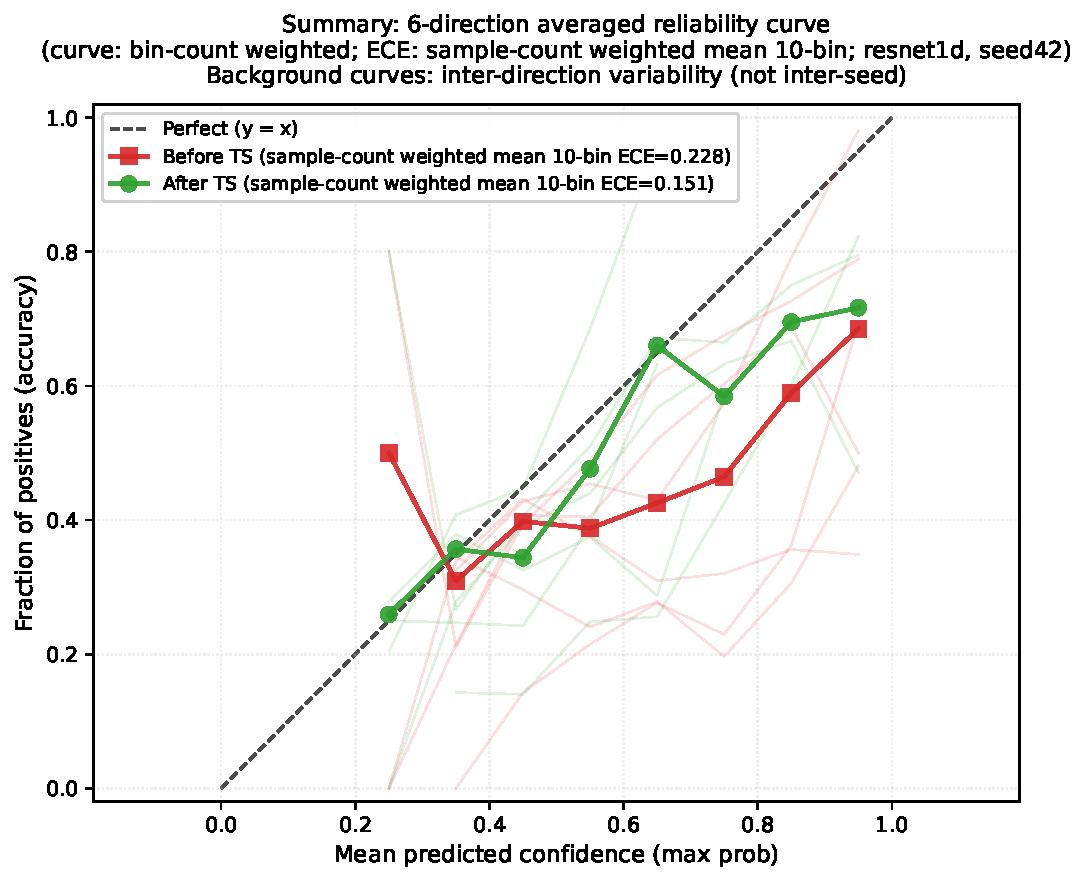
\includegraphics[width=0.95\columnwidth]{figures/fig_reliability_summary.pdf}
\caption{汇总可靠性曲线：6 方向分箱计数加权
平均。样本计数加权均值 ECE 在
温度缩放后从 $\text{ECE}_{\text{raw}}$ 降至 $\text{ECE}_{\text{TS}}$。
淡色背景曲线展示个别
方向变异性。}
\label{fig:reliability-summary}
\end{figure}

\begin{figure}[t]
\centering
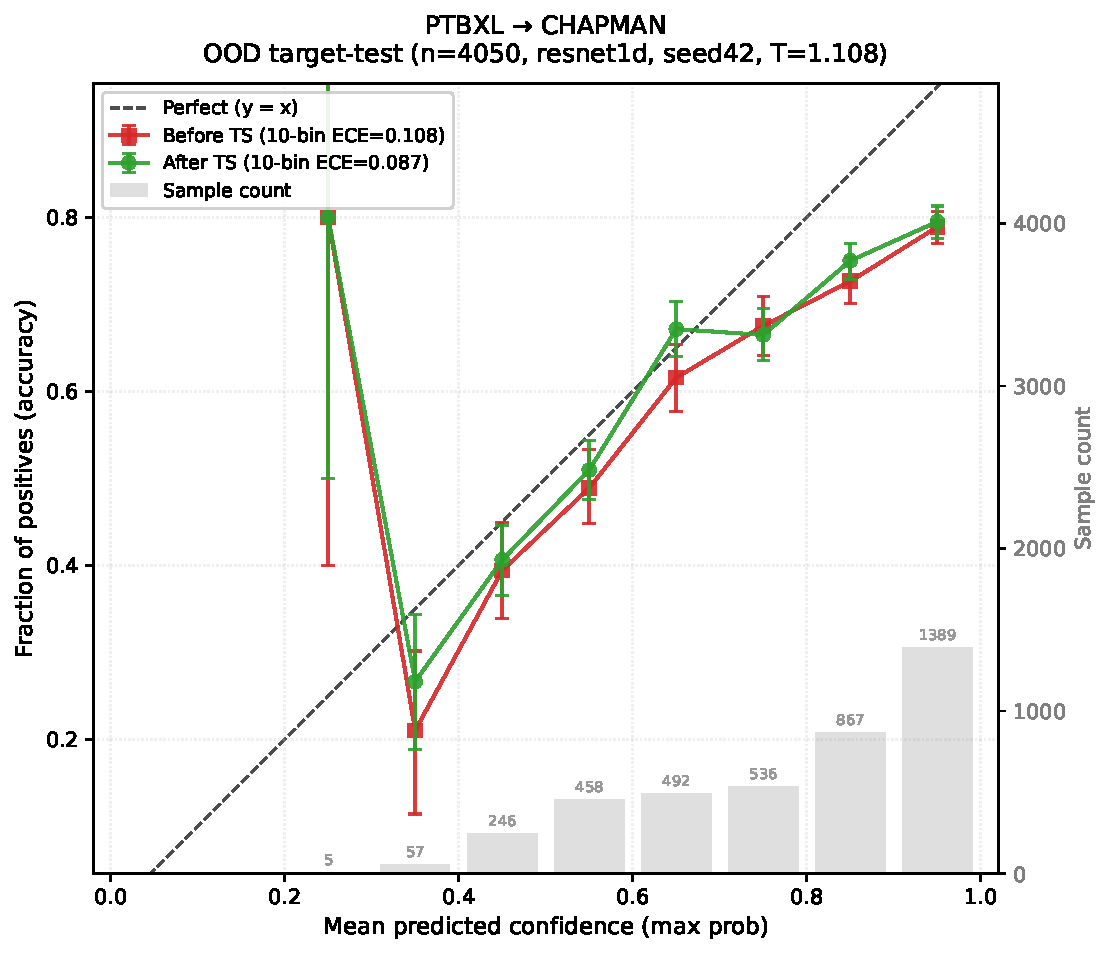
\includegraphics[width=0.48\columnwidth]{figures/fig_reliability_ptbxl_chapman.pdf}
\hfill
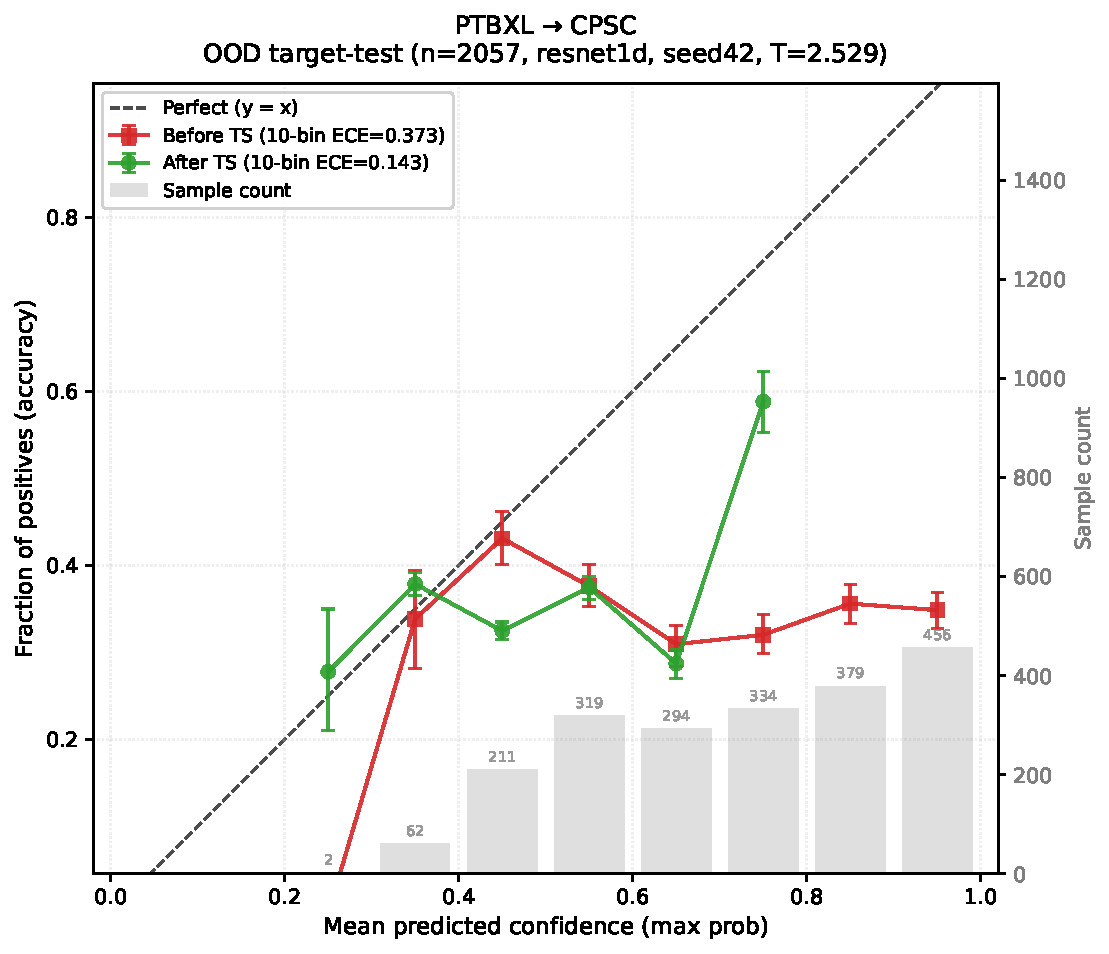
\includegraphics[width=0.48\columnwidth]{figures/fig_reliability_ptbxl_cpsc.pdf}
\caption{PTB-XL$\to$Chapman（左）和
PTB-XL$\to$CPSC（右）的可靠性图。OOD 目标测试集，ResNet1D，种子~42。}
\label{fig:rel-ptbxl-chapman}
\end{figure}

\begin{figure}[t]
\centering
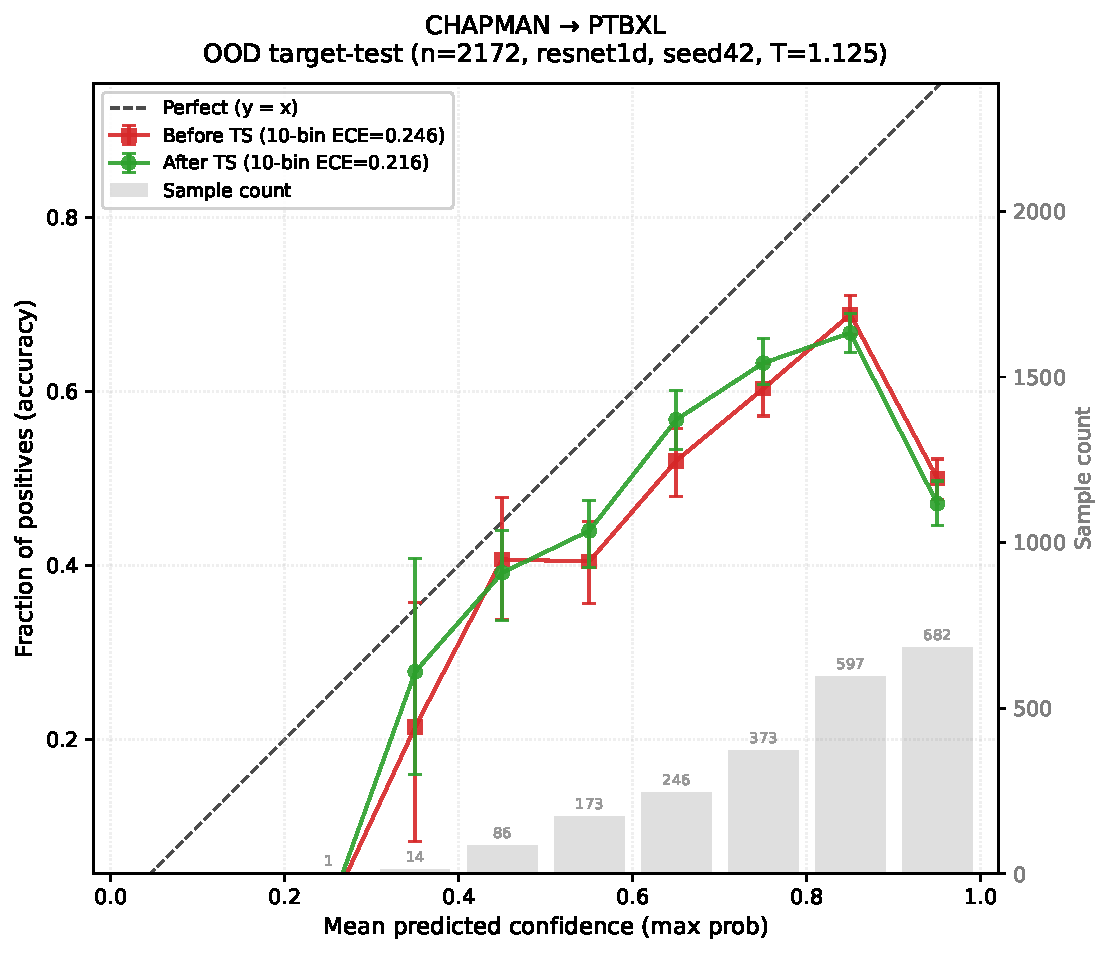
\includegraphics[width=0.48\columnwidth]{figures/fig_reliability_chapman_ptbxl.pdf}
\hfill
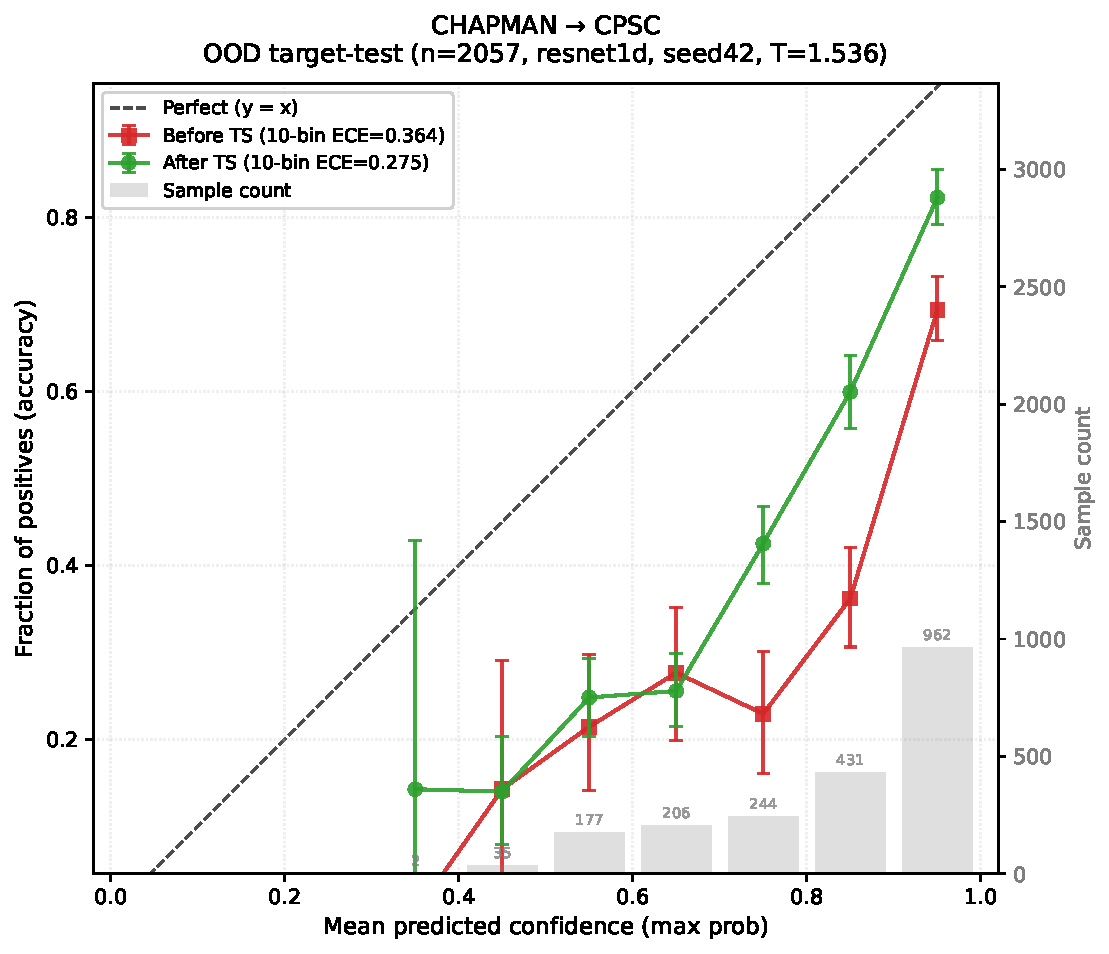
\includegraphics[width=0.48\columnwidth]{figures/fig_reliability_chapman_cpsc.pdf}
\caption{Chapman$\to$PTB-XL（左）和
Chapman$\to$CPSC（右）的可靠性图。OOD 目标测试集，ResNet1D，种子~42。}
\label{fig:rel-chapman-ptbxl}
\end{figure}

\begin{figure}[t]
\centering
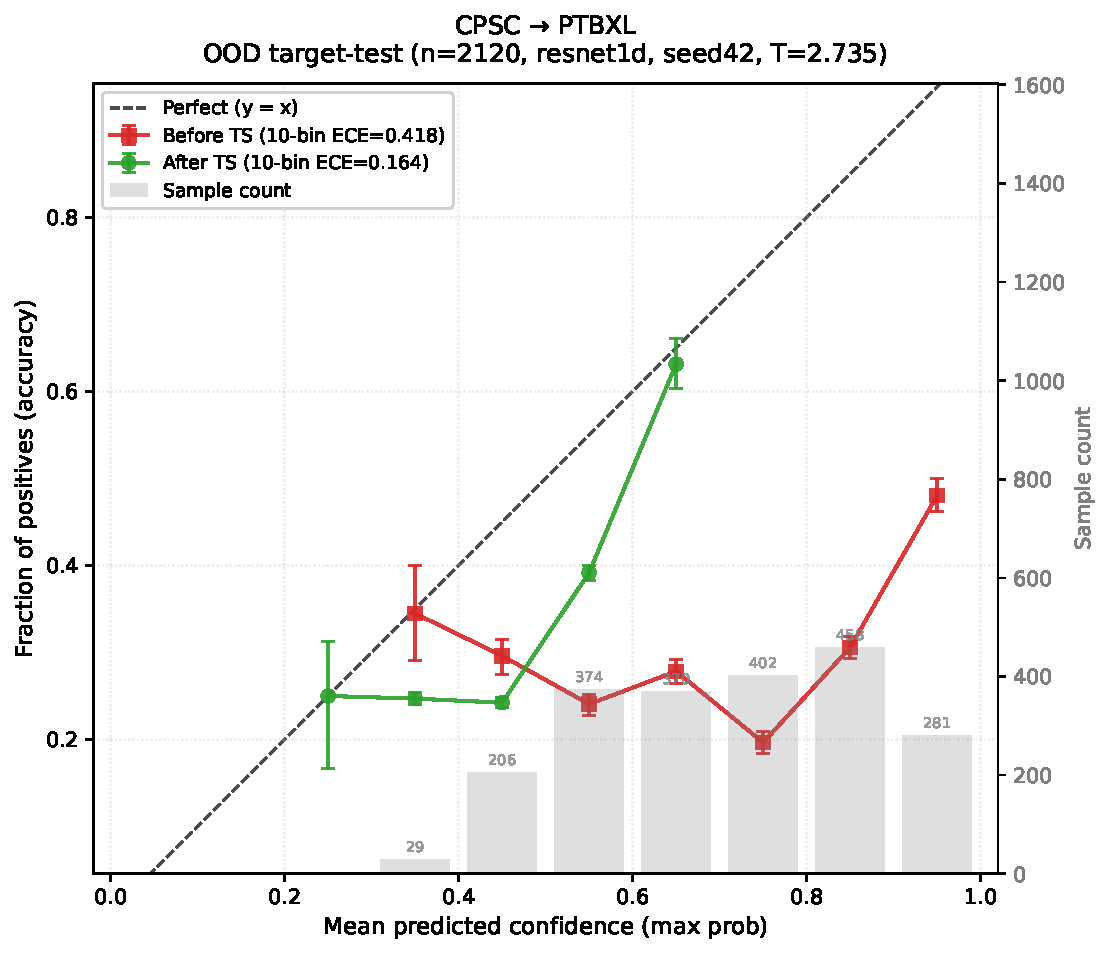
\includegraphics[width=0.48\columnwidth]{figures/fig_reliability_cpsc_ptbxl.pdf}
\hfill
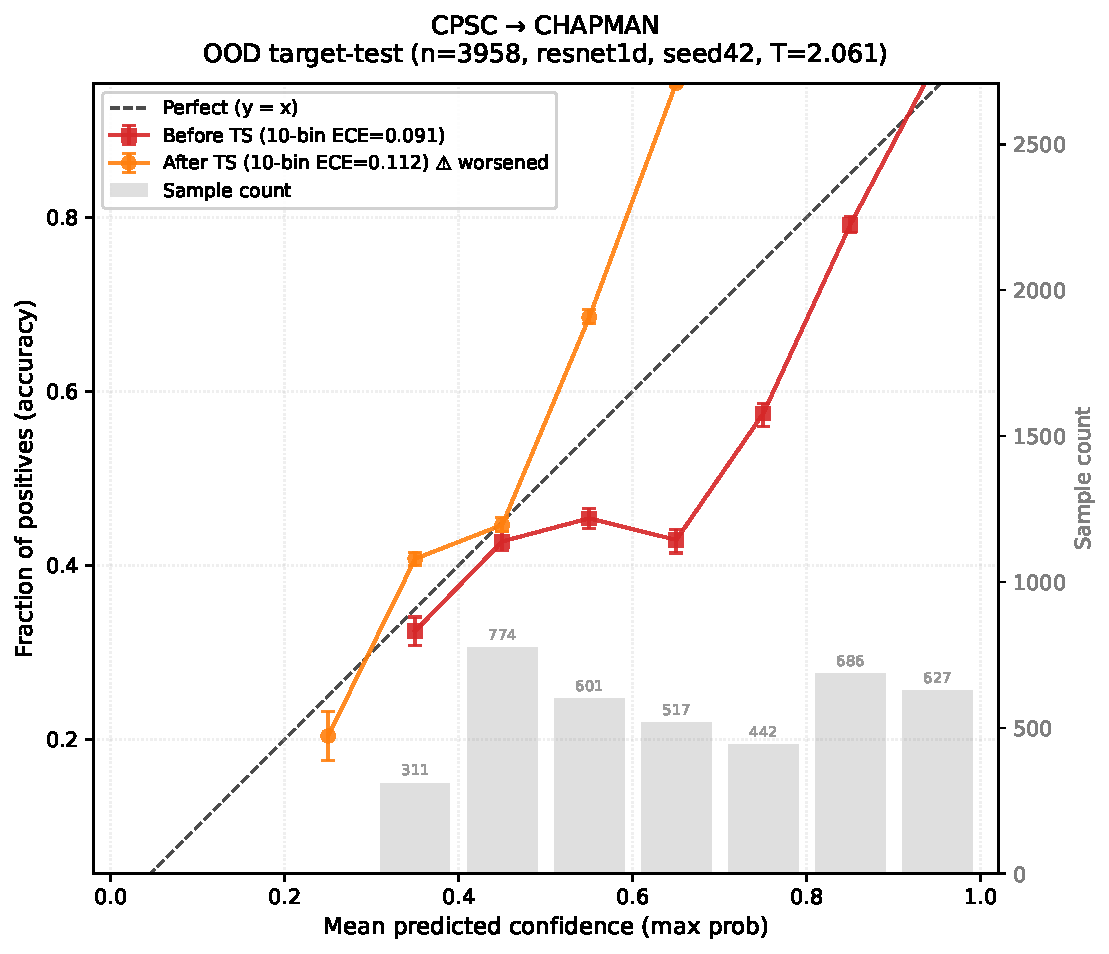
\includegraphics[width=0.48\columnwidth]{figures/fig_reliability_cpsc_chapman.pdf}
\caption{CPSC$\to$PTB-XL（左）和
CPSC$\to$Chapman（右）的可靠性图。OOD 目标测试集，ResNet1D，种子~42。}
\label{fig:rel-cpsc-chapman}
\end{figure}

